\documentclass[journal]{IEEEtran}

\usepackage[spanish,es-tabla,es-noshorthands]{babel}
\usepackage[utf8]{inputenc}
\usepackage[T1]{fontenc}
\usepackage[pdftex]{graphicx}
\usepackage{cite}
\usepackage{array}
\usepackage{url}
\usepackage{amsmath}
\makeatletter\newcommand{\captionof}[1]{\def\@captype{#1}\caption}\makeatother
\renewcommand{\ttdefault}{lmtt}
\usepackage{xcolor}
\usepackage{float}
\floatstyle{ruled}
\newcommand{\al}[2]{\par\noindent\hangindent=\dimexpr#1em+1.6em\relax\hangafter=1\hspace*{#1em}\li#2}
\newcounter{lin}\newcommand{\li}{\stepcounter{lin}\thelin:\ }
\newfloat{algoritmo}{tbp}{loa}
\floatname{algoritmo}{Algoritmo}
\addto\captionsspanish{\renewcommand{\appendixname}{Anexo}}

\newcommand{\notatabla}[1]{\par\vspace{4pt}\colorbox{gray!12}{\parbox{\dimexpr\linewidth-2\fboxsep\relax}{\footnotesize\raggedright #1}}}

\graphicspath{{../../}}
\hyphenation{per-mu-ta-tion flow-shop makes-pan fe-ro-mo-na}

\begin{document}
\raggedbottom

\title{Comparing a Genetic Algorithm, a Memetic Algorithm, an Ant Colony System and Extremal Optimization for the Permutation Flow Shop Problem}
\author{Cristóbal Alvarado, Benjamín Bizama y Benjamín Jeldres%
\thanks{Cristóbal Alvarado, Benjamín Bizama y Benjamín Jeldres pertenecen al Departamento de Ingeniería Informática, Facultad de Ingeniería, Universidad Católica de la Santísima Concepción, Concepción, Chile. Contacto: \{calvarado, bbizama, bjeldres\}@ing.ucsc.cl.}}

\markboth{Informe de investigación, noviembre de 2026}{Alvarado, Bizama y Jeldres: AG, AM, ACS y EO para el PFSP}
\maketitle

\begin{otherlanguage}{english}
  \begin{abstract}
    The permutation flow shop problem asks for the sequence of $n$ jobs on $m$ machines that minimizes the makespan. Four metaheuristics share that encoding and the same evaluator: a genetic algorithm (AG), a memetic algorithm (AM) that adds one pass of insertion local search to the AG, an ant colony system (ACS), and $\tau$-extremal optimization (EO). Quality is the relative percentage deviation from the upper bound published with each instance. Three Taillard instances, of sizes $20\times5$, $50\times10$ and $100\times10$, were solved with 30 seeds. The base budget is 10\,000 makespan evaluations, and the design is 4 algorithms $\times$ 3 instances $\times$ 30 seeds, that is 360 runs. The analysis is descriptive. The AM records the lowest mean deviation on every instance (1.38\%, 3.57\% and 1.38\%) and is the only method that matches a published bound, twice on the smallest instance. On $100\times10$ the AM spends 210\,020 evaluations and 147.6\,s of CPU time, against 10\,000 evaluations and 8.0\,s for the AG. Without local search, the ACS and the EO stay above the AG. A shortest-processing-time sequence and the mean of 1\,000 random permutations are reported as baselines.
  \end{abstract}
\end{otherlanguage}

\begin{IEEEkeywords}
  Permutation flow shop, makespan, genetic algorithm, memetic algorithm, ant colony system, extremal optimization, Taillard instances.
\end{IEEEkeywords}

\section{Introducción}\label{sec:introduccion}
\IEEEPARstart{E}{n} un taller en línea, el orden de entrada de los trabajos decide cuánto esperan las máquinas y cuándo termina el lote. El \textit{Permutation Flow Shop Problem} (PFSP) exige que $n$ trabajos visiten $m$ máquinas en el mismo orden tecnológico y que la secuencia de entrada se conserve en todas ellas. El objetivo de este estudio es minimizar el \textit{makespan}, el instante en que termina el último trabajo, $C_{\max}$.\footnote{$C_{\max}$ es la notación estándar del \textit{makespan}: si $C_j$ es el instante en que el trabajo $j$ termina su última operación, $C_{\max}=\max_j C_j$. Menor $C_{\max}$ significa mejor solución.}

El problema es NP-\textit{hard} para tres o más máquinas \cite{garey_complexity_1976}. Algunas instancias de Taillard \cite{taillard_benchmarks_1993} se cerraron recién en 2022 con supercomputadores \cite{gmys_exactly_2022}. Por eso se comparan metaheurísticas. La heurística constructiva NEH (Nawaz--Enscore--Ham) arma una solución sin azar: ordena los trabajos por tiempo total decreciente e inserta cada uno, en ese orden, en la posición de menor \textit{makespan} parcial; sigue siendo la referencia clásica \cite{nawaz_heuristic_1983,ruiz_comprehensive_2005}. Los algoritmos genéticos evolucionan un conjunto de soluciones (una población) combinándolas y alterándolas al azar, y se aplicaron al PFSP desde los noventa \cite{reeves_genetic_1995}. Un algoritmo memético les agrega búsqueda local: prueba pequeñas variaciones de una solución prometedora e intenta mejorarla \cite{moscato_evolution_1989}. El sistema de colonia de hormigas construye secuencias guiado por la feromona, una memoria numérica compartida que marca qué decisiones dieron buenas soluciones \cite{dorigo_ant_1997,dorigo_ant_2004} y ya se adaptó al PFSP \cite{stutzle_ant_1998,rajendran_ant-colony_2004}. La optimización extremal ($\tau$-EO) trabaja con una sola solución: elige, con una ley de potencia, un componente mal ubicado, lo cambia y acepta el resultado aunque empeore \cite{boettcher_natures_2000,boettcher_optimization_2001}.

El equipo ya comparó un algoritmo genético y uno memético cuya población inicial incluía una solución NEH \cite{equipo_ag_neh_2026} (se dice que la población está \emph{sembrada}), y validó un sistema de colonia de hormigas sobre Berlin52 \cite{equipo_acs_tsp_2026}. Este informe no siembra ninguna solución. Compara cuatro implementaciones concretas, con el mismo evaluador y un presupuesto común de 10\,000 evaluaciones de \textit{makespan}. No pretende aislar la contribución pura de cada familia de métodos, porque cada uno conserva sus operadores y sus parámetros.

La Sección~\ref{sec:marco} resume los cuatro métodos. La Sección~\ref{sec:metodo} formula el PFSP y describe cada algoritmo. La Sección~\ref{sec:diseno} fija instancias, presupuesto y entorno. La Sección~\ref{sec:resultados} informa calidad, costo y líneas de base. La Sección~\ref{sec:conclusiones} cierra.

\section{Marco teórico}\label{sec:marco}
Antes de describir los métodos conviene fijar los términos que comparten. Una \emph{solución} es una secuencia de trabajos (una permutación). Una \emph{población} es un conjunto de $N$ soluciones que evolucionan juntas; cada una es un \emph{individuo}, y cada paso del ciclo que produce una población nueva es una \emph{generación}. La \emph{selección} escoge individuos para reproducirse, con preferencia por los de menor $C_{\max}$. El \emph{cruce} combina dos padres en un hijo que hereda partes de ambos. La \emph{mutación} altera un individuo al azar y mantiene la diversidad. La \emph{aptitud} de una solución es qué tan buena es; aquí, su $C_{\max}$. La \emph{búsqueda local} parte de una solución, prueba soluciones \emph{vecinas} (aquí, las que resultan de mover un trabajo a otra posición) y se queda con una mejor, si existe. El \emph{elitismo} conserva siempre la mejor solución encontrada. Se llama \emph{explotación} a refinar lo que ya parece bueno y \emph{exploración} a probar zonas nuevas.

Los cuatro métodos usan decisiones aleatorias (qué padres, dónde cortar, qué trabajo mover). La \emph{semilla} es el valor inicial del generador de números pseudoaleatorios: con la misma semilla, instancia y parámetros, una corrida repite exactamente la misma secuencia de decisiones y el mismo resultado. Semillas distintas dan corridas independientes, y por eso se repite cada experimento con 30 semillas. No confundir con \emph{sembrar} una población, que es insertar una solución conocida en la población inicial.

Un algoritmo genético (AG) mantiene una población de soluciones. En cada generación selecciona padres, los combina, los perturba y reemplaza a la población. La presión selectiva decide cuánto pesa la calidad frente a la diversidad.

Un algoritmo memético (AM) es ese ciclo más una búsqueda local. La solución mejorada reemplaza al individuo que la originó, de modo que el resultado de la explotación vuelve a la población y puede heredarse.

La optimización por colonia de hormigas construye soluciones paso a paso. Cada \emph{hormiga} parte de un trabajo y elige cuál va después. Una decisión ``el trabajo $j$ va justo después del $i$'' es una \emph{arista}, y cada arista tiene un valor de \emph{feromona}: un número que sube cuando esa decisión aparece en buenas soluciones y que guía a las hormigas siguientes. La \emph{evaporación} baja ese valor con el tiempo para olvidar decisiones antiguas. La \emph{visibilidad} es información fija del problema que también orienta la elección (aquí, preferir trabajos cortos). En el sistema de colonia de hormigas (ACS, \textit{ant colony system}), cada hormiga elige con probabilidad $q_0$ la mejor arista según feromona y visibilidad (explotación) y, si no, sortea entre las aristas con probabilidad proporcional a ese valor, como una \emph{ruleta} donde cada arista ocupa un sector más ancho cuanto mejor es. Además, cada arista que una hormiga recorre pierde parte de su feromona (evaporación local), para que las siguientes prueben otras; y al final solo se refuerza la mejor solución conocida \cite{dorigo_ant_1997}.

La optimización extremal (EO, \textit{extremal optimization}) mantiene una sola solución y siempre modifica sus componentes menos adecuados. Parte del modelo de Bak y Sneppen, en el que se reemplaza la especie de peor aptitud y el sistema se acerca a un estado crítico \cite{bak_punctuated_1993}. Boettcher y Percus la convierten en $\tau$-EO: se ordenan los componentes de peor a mejor aptitud y se elige el de rango $k$ con probabilidad proporcional a $k^{-\tau}$ \cite{boettcher_natures_2000,boettcher_optimization_2001}. El cambio se acepta siempre y se guarda el mejor estado visto. Para varios problemas proponen $\tau\approx 1+1/\ln n$. Aquí no se calibra $\tau$.

\section{Metodología}\label{sec:metodo}
\subsection{Permutation Flow Shop Problem}
Sea $\pi=(\pi_1,\ldots,\pi_n)$ la secuencia de trabajos. $C(i,j)$ es el instante en que termina el trabajo que ocupa la posición $i$ de $\pi$ en la máquina $j$:
\begin{equation}
  C(i,j)=\max\{C(i-1,j),\,C(i,j-1)\}+p_{\pi_i,j},\label{eq:cmax}
\end{equation}
con $C(0,j)=C(i,0)=0$ y $p_{\pi_i,j}$ el tiempo de ese trabajo en esa máquina. El \textit{makespan} es $C_{\max}(\pi)=C(n,m)$.

La cota superior (UB, \textit{upper bound}) es el valor publicado por Taillard en 1993 para cada instancia \cite{taillard_benchmarks_1993}. No es, por sí sola, un óptimo demostrado: en tamaños grandes hay soluciones posteriores mejores \cite{gmys_exactly_2022,brunner_permutation_2025}. La desviación porcentual relativa (RPD) mide cuánto supera un resultado a esa cota:
\begin{equation}
  \mathrm{RPD}(\%)=100\cdot\frac{C_{\max}-C_{\max}^{\mathrm{UB}}}{C_{\max}^{\mathrm{UB}}}.\label{eq:rpd}
\end{equation}
Un RPD de 0\% iguala la UB. Un RPD negativo la mejora.

\subsection{Algoritmo genético}
El AG (Algoritmo~\ref{alg:ag}) hace evolucionar una población de $N$ secuencias durante $T$ generaciones. Funciona así:
\begin{itemize}
  \item \textbf{Inicio:} la población parte con $N$ secuencias al azar de los trabajos $0,\ldots,n-1$. Se calcula el $C_{\max}$ de cada una.
  \item \textbf{Elegir padres:} por torneo. Se sortean 3 individuos y gana el de menor $C_{\max}$. Se repite para el segundo padre.
  \item \textbf{Cruce} (con probabilidad $p_c$): el hijo copia un tramo del primer padre en su misma posición y completa el resto con los demás trabajos, en el orden en que aparecen en el segundo padre (OX, \textit{order crossover} \cite{davis_applying_1985}). Si no hay cruce, el hijo es una copia del primer padre.
  \item \textbf{Mutación} (con probabilidad $p_m$): se saca un trabajo del hijo y se inserta en otra posición.
  \item \textbf{Nueva población:} los $N$ hijos reemplazan a la población anterior. Antes, el mejor individuo encontrado hasta ahora (elitismo) ocupa el lugar del peor hijo, así que el mejor $C_{\max}$ nunca empeora.
\end{itemize}

\begin{algoritmo}[H]
  \caption{Algoritmo genético (AG).}\label{alg:ag}
  \footnotesize\setcounter{lin}{0}
  \al{0}{Generar una población inicial de $N$ permutaciones aleatorias}
  \al{0}{Evaluar $C_{\max}$ de cada individuo de la población inicial}
  \al{0}{\textbf{while} no se cumpla la condición de término ($T$ generaciones) \textbf{do}}
  \al{1}{\textbf{for} un tamaño predeterminado de población ($N$ hijos) \textbf{do}}
  \al{2}{Seleccionar dos padres por torneo de 3 individuos}
  \al{2}{Aplicar el operador de cruce OX a los padres con probabilidad $p_c$ para generar el hijo (si no, el hijo copia al primer padre)}
  \al{2}{Aplicar el operador de mutación por inserción al hijo con probabilidad $p_m$}
  \al{2}{Evaluar $C_{\max}$ del hijo}
  \al{1}{\textbf{end for}}
  \al{1}{Generar una nueva población con los $N$ hijos; el mejor individuo histórico reemplaza al peor hijo}
  \al{0}{\textbf{end while}}
  \al{0}{\textbf{return} la mejor solución encontrada}
\end{algoritmo}

\subsection{Algoritmo memético}
El AM (Algoritmo~\ref{alg:am}) es el mismo AG con un paso más: cada $f_{BL}$ generaciones toma al mejor individuo y trata de mejorarlo con búsqueda local. La búsqueda local prueba cada trabajo en todas las posiciones de la secuencia y lo deja en la mejor, solo si el $C_{\max}$ baja. El individuo mejorado reemplaza al original. Cuesta $n^2+1$ evaluaciones: la secuencia de entrada y un \textit{makespan} por inserción candidata. En los experimentos $f_{BL}=10$, el valor del ejemplo de la sección 5 del enunciado, así que en 200 generaciones hay 20 búsquedas locales.

\begin{algoritmo}[H]
  \caption{Algoritmo memético (AM).}\label{alg:am}
  \footnotesize\setcounter{lin}{0}
  \al{0}{Generar una población inicial de $N$ permutaciones aleatorias}
  \al{0}{Evaluar $C_{\max}$ de cada individuo de la población inicial}
  \al{0}{\textbf{while} no se cumpla la condición de término ($T$ generaciones) \textbf{do}}
  \al{1}{\textbf{for} un tamaño predeterminado de población ($N$ hijos) \textbf{do}}
  \al{2}{Seleccionar dos padres por torneo de 3 individuos}
  \al{2}{Aplicar el operador de cruce OX a los padres con probabilidad $p_c$ para generar el hijo (si no, el hijo copia al primer padre)}
  \al{2}{Aplicar el operador de mutación por inserción al hijo con probabilidad $p_m$}
  \al{2}{Evaluar $C_{\max}$ del hijo}
  \al{1}{\textbf{end for}}
  \al{1}{Generar una nueva población con los $N$ hijos; el mejor individuo histórico reemplaza al peor hijo}
  \al{1}{\textbf{if} la generación es múltiplo de $f_{BL}$ \textbf{then}}
  \al{2}{Aplicar búsqueda local por inserción al mejor individuo de la población, y reemplazarlo por el resultado}
  \al{1}{\textbf{end if}}
  \al{0}{\textbf{end while}}
  \al{0}{\textbf{return} la mejor solución encontrada}
\end{algoritmo}

\subsection{Sistema de colonia de hormigas}
Cada iteración construye $N$ secuencias. Cada hormiga parte de un trabajo al azar y agrega trabajos hasta completar la permutación. Al terminar la iteración se refuerza la mejor secuencia global (Algoritmo~\ref{alg:acs}).

Se conservó el esquema del ACS usado en Berlin52 \cite{equipo_acs_tsp_2026}: la regla pseudoaleatoria proporcional, la actualización local en cada arista y el refuerzo global solo de la mejor solución, con el mismo factor $\alpha$ en ambas. Se adaptaron la representación y la información del problema. La matriz $\tau$ es dirigida, porque programar $j$ después de $i$ no equivale al revés, y la secuencia no se cierra. La visibilidad es la regla SPT (\textit{shortest processing time}), $\eta_j=1/\sum_k p_{j,k}$. La feromona inicial es $\tau_0=1/(n\cdot C_{\max}^{\mathrm{SPT}})$, con $C_{\max}^{\mathrm{SPT}}$ el \textit{makespan} de ordenar los trabajos por tiempo total creciente. El objetivo es $C_{\max}$, no el largo de un ciclo.

Desde el trabajo $i$, sobre los trabajos pendientes $\mathcal{U}$,
\begin{equation}
  j=
  \begin{cases}
    \arg\max_{u\in\mathcal{U}}\tau_{iu}\,\eta_u^{\beta} & \text{si } q\leq q_0,\\[4pt]
    \text{ruleta con } P_{ij}\propto \tau_{ij}\,\eta_j^{\beta} & \text{si } q>q_0,
  \end{cases}\label{eq:transicion}
\end{equation}
con $q$ uniforme en $(0,1)$. La actualización local es
\begin{equation}\tau_{ij}\leftarrow(1-\alpha)\tau_{ij}+\alpha\tau_0.\label{eq:local}\end{equation} Con $0<\alpha<1$ el valor nuevo es una combinación convexa de $\tau_{ij}$ y $\tau_0$: baja si $\tau_{ij}>\tau_0$, no cambia si son iguales y sube si $\tau_{ij}<\tau_0$. No disminuye siempre. La actualización global, solo en las aristas de $\pi^{*}$, es
\begin{equation}\tau_{ij}\leftarrow(1-\alpha)\tau_{ij}+\alpha/C_{\max}(\pi^{*}).\label{eq:global}\end{equation}

\begin{algoritmo}[H]
  \caption{Sistema de colonia de hormigas (ACS).}\label{alg:acs}
  \footnotesize\setcounter{lin}{0}
  \al{0}{Inicializar la feromona en todos los segmentos ($\tau_{ij}\leftarrow\tau_0$)}
  \al{0}{\textbf{while} no se cumpla la condición de término ($T$ iteraciones) \textbf{do}}
  \al{1}{\textbf{for} cada hormiga \textbf{do}}
  \al{2}{Asignar randómicamente la hormiga a un trabajo (vértice) del grafo}
  \al{2}{\textbf{for} cada trabajo restante \textbf{do}}
  \al{3}{Seleccionar el próximo trabajo usando la Ecuación~\eqref{eq:transicion}}
  \al{3}{Actualizar la feromona del segmento recorrido según la Ecuación~\eqref{eq:local}}
  \al{2}{\textbf{end for}}
  \al{2}{Evaluar $C_{\max}$ de la secuencia construida}
  \al{1}{\textbf{end for}}
  \al{1}{\textbf{if} es encontrada una mejor solución en la iteración actual \textbf{then}}
  \al{2}{Actualizar la mejor solución del proceso hasta la iteración actual}
  \al{1}{\textbf{end if}}
  \al{1}{Actualizar la feromona en los segmentos de la mejor solución según la Ecuación~\eqref{eq:global}}
  \al{0}{\textbf{end while}}
  \al{0}{\textbf{return} la mejor solución global}
\end{algoritmo}

\subsection{Optimización extremal}
$\tau$-EO mantiene una sola permutación. En cada iteración mide el \textit{makespan} y el ocio de cada posición en la misma pasada. El ocio de la posición $i$ es
\begin{equation}
  o_i=\sum_{j=2}^{m}\max\bigl(0,\,C(i,j-1)-C(i-1,j)\bigr).\label{eq:ocio}
\end{equation}
Es el tiempo que la posición hace esperar a las máquinas $2,\ldots,m$. Se ordenan las posiciones de mayor a menor ocio. El rango $k=1$ es la peor. Los empates se rompen al azar. Se elige una posición con $P(k)\propto k^{-\tau}$ y ese trabajo se inserta en otra posición, el mismo movimiento que la mutación del AG. El estado nuevo se acepta siempre. Se guardan la mejor permutación y su $C_{\max}$. El Algoritmo~\ref{alg:eo} resume el ciclo.

\begin{algoritmo}[H]
  \caption{$\tau$-EO.}\label{alg:eo}
  \footnotesize\setcounter{lin}{0}
  \al{0}{Generar una solución inicial aleatoria $\pi$ (permutación de los trabajos)}
  \al{0}{$\pi^{*}\leftarrow\pi$}
  \al{0}{Generar el arreglo de probabilidades $P_k\propto k^{-\tau}$, $1\le k\le n$}
  \al{0}{\textbf{for} un número predeterminado de iteraciones ($T$) \textbf{do}}
  \al{1}{Evaluar $C_{\max}(\pi)$ y el ocio $o_i$ de cada posición (Ecuación~\eqref{eq:ocio}), y ordenar las posiciones de peor (mayor ocio) a mejor, con empates al azar}
  \al{1}{\textbf{if} $C_{\max}(\pi)<C_{\max}(\pi^{*})$ \textbf{then} $\pi^{*}\leftarrow\pi$}
  \al{1}{Seleccionar la posición $s$ según la probabilidad $P_k$ de su rango $k$}
  \al{1}{Insertar el trabajo $\pi_s$ en otra posición al azar (el cambio se acepta siempre)}
  \al{0}{\textbf{end for}}
  \al{0}{\textbf{return} $\pi^{*}$ y $C_{\max}(\pi^{*})$}
\end{algoritmo}

\subsection{Decisiones de diseño}
Estas elecciones no se compararon entre sí en este estudio. No se presentan como superioridad demostrada.
\begin{itemize}
  \item Torneo $k=3$ y no ruleta. La ruleta, al minimizar, exige transformar $C_{\max}$. Si los valores de la población son parecidos, las probabilidades quedan casi planas. El torneo solo compara.
  \item OX y no PMX. PMX (\textit{partially mapped crossover}) conserva posiciones absolutas mediante un mapeo. OX conserva un bloque y el orden relativo del otro padre. El $C_{\max}$ depende de ese orden. No se ejecutó PMX.
  \item Inserción y no intercambio. La inserción mueve un trabajo y deja el orden del resto. Es el vecindario de NEH \cite{nawaz_heuristic_1983}.
  \item Un elitista, no el reemplazo $(\mu+\lambda)$ del informe anterior \cite{equipo_ag_neh_2026}. En $(\mu+\lambda)$ compiten padres e hijos y sobreviven los mejores. El enunciado pide reemplazo generacional con elitismo. Conservar un individuo basta para que el mejor $C_{\max}$ no empeore.
  \item Búsqueda local por inserción, una pasada, solo al mejor, cada $f_{BL}=10$ generaciones. Aplicarla a toda la población multiplicaría el costo por $N$. No se usó 2-opt: invertir un tramo invierte sus precedencias.
  \item Visibilidad SPT y no una basada en NEH. NEH dentro de $\eta$ mezclaría una heurística constructiva fuerte con la colonia. SPT se calcula una vez.
  \item $\tau=1.4$, el valor del ejemplo de la sección 5 del enunciado. La regla $\tau\approx 1+1/\ln n$ da cerca de 1.33, 1.26 y 1.22 para $n=20$, 50 y 100 \cite{boettcher_optimization_2001}. No se barrió $\tau$.
\end{itemize}

\section{Diseño experimental}\label{sec:diseno}
\subsection{Instancias, semillas y presupuesto}
Se usó la primera instancia de Taillard de cada tamaño pedido: ta001 ($20\times5$, UB 1278), ta041 ($50\times10$, UB 3025) y ta071 ($100\times10$, UB 5770). La semilla del encabezado de cada archivo coincide con la de Taillard \cite{taillard_benchmarks_1993}. La UB es la cota de 1993, definida en la Sección~\ref{sec:metodo}. En ta001 coincide con el óptimo conocido; en las otras dos no es un certificado.

Hay cuatro algoritmos, tres instancias y las semillas 1 a 30. El total es $4\times 3\times 30=360$ corridas. El análisis es descriptivo: no hay pruebas de hipótesis. Treinta semillas estiman mejor la dispersión que diez; no garantizan significancia.

El presupuesto base es 10\,000 evaluaciones de $C_{\max}$. El AG y el ACS lo gastan como 50 individuos u hormigas por 200 iteraciones. EO hace 10\,000 iteraciones, una evaluación cada una, y registra una fila cada 50. El AM suma $n^2+1$ evaluaciones por cada una de sus 20 pasadas de búsqueda local. La población inicial del AG y el \textit{makespan} SPT que fija $\tau_0$ no entran en esa cuenta. La comparación iguala el presupuesto base, no el total de evaluaciones ni el tiempo. La Tabla~\ref{tab:tiempo} muestra las tres magnitudes.

\subsection{Parámetros}
La Tabla~\ref{tab:parametros} lista los valores. El presupuesto, $p_c=0.8$, $p_m=0.1$, $f_{BL}=10$ y $q_0=0.9$ salen del ejemplo de ejecución de la sección 5 del enunciado. $q_0=0.9$ es también el valor de Dorigo y Gambardella \cite{dorigo_ant_1997}. Esos valores no se calibraron. Del ejemplo del ACS se cambiaron dos: $\alpha=0.1$ en lugar de 1.0, porque $\alpha=1$ reemplaza toda la feromona en cada actualización, y $\beta=1.0$ en lugar de 2.0. En ta001, con cinco semillas, el RPD medio del ACS fue 3.19\% ($\beta=0$), 2.90\% ($\beta=1$), 3.35\% ($\beta=2$) y 5.60\% ($\beta=5$). Esa prueba usa una instancia que después se evalúa, así que favorece levemente al ACS en $20\times5$.

\begin{table}[!t]
  \caption{Parámetros. El origen es la sección 5 del enunciado, salvo $\alpha$ y $\beta$.}\label{tab:parametros}
  \centering\footnotesize
  \begin{tabular}{l l}\hline
    Alcance & Valores\\ \hline
    Común & 10\,000 evaluaciones base, semillas 1--30\\
    AG & $N=50$, $p_c=0.8$, $p_m=0.1$, torneo $k=3$\\
    AM & los del AG y $f_{BL}=10$\\
    ACS & $N=50$, $\alpha=0.1$, $\beta=1.0$, $q_0=0.9$\\
    EO & 10\,000 iteraciones, $\tau=1.4$\\ \hline
  \end{tabular}
  \notatabla{$N$: individuos u hormigas. $p_c$, $p_m$: probabilidad de cruce y de mutación. $f_{BL}$: generaciones entre búsquedas locales. $\alpha$: peso de la actualización de feromona. $\beta$: peso de la visibilidad. $q_0$: umbral de explotación en \eqref{eq:transicion}. $\tau$: exponente de la ley de potencia.}
\end{table}

\subsection{Implementación, entorno y pruebas}
El código está en Python~3. Cada algoritmo vive en su programa (\texttt{ag.py}, \texttt{am.py}, \texttt{acs.py}, \texttt{eo.py}). \texttt{am.py} llama al ciclo del AG con $f_{BL}>0$. \texttt{operadores.py} lee instancias, calcula $C_{\max}$ y el ocio, y aplica los operadores. \texttt{main.py} arma las 360 tareas y las reparte con un \texttt{ProcessPoolExecutor}. El tamaño del pool es el número de CPUs asignadas al proceso.

Las corridas se hicieron en el servidor Jupyter del curso, respaldado por Slurm. El tiempo informado es tiempo de CPU por corrida (\texttt{time.process\_time}), no el reloj de pared del pool: no cambia porque otras corridas compartan la máquina.

Hay pruebas automáticas, no solo aserciones sueltas. Un caso con resultado calculado a mano usa tres trabajos y dos máquinas, con tiempos $(3,2)$, $(1,4)$ y $(2,1)$. La secuencia $(0,1,2)$ debe dar $C_{\max}=10$ y ocio $(3,0,0)$. La secuencia $(1,0,2)$ debe dar $C_{\max}=8$. La misma batería de pruebas exige permutaciones válidas, que el mejor $C_{\max}$ de AG, AM, ACS y EO no empeore, y que una semilla repetida devuelva la misma secuencia. El $C_{\max}$ de una secuencia de ta001 se contrastó con la implementación del informe anterior \cite{equipo_ag_neh_2026}: ambos dan 1286.

\section{Resultados}\label{sec:resultados}
\subsection{Calidad}
La Tabla~\ref{tab:calidad} resume 30 semillas por celda. En las tres instancias el menor RPD medio (columna RPD medio) es el del AM: 1.38\%, 3.57\% y 1.38\%. El AG queda segundo (1.55\%, 5.76\% y 4.83\%). El ACS y EO quedan después. EO es levemente peor que el ACS en $20\times5$ (3.60\% frente a 3.28\%) y en $100\times10$ (11.24\% frente a 9.84\%), y levemente mejor en $50\times10$ (13.89\% frente a 14.15\%).

\begin{table*}[!t]
  \caption{Calidad sobre 30 semillas.}\label{tab:calidad}
  \centering\footnotesize
  \begin{tabular}{l l r r c c c}\hline
    Instancia & Alg. & Mejor & Media $\pm$ desv. & RPD medio & RPD mín.--máx. & En UB\\ \hline
    ta001 $20\times5$ & AG & 1297 & $1297.8\pm 4.6$ & 1.55 & 1.49--3.44 & 0/30\\
    UB 1278 & AM & \textbf{1278} & $1295.7\pm 6.2$ & \textbf{1.38} & 0.00--2.11 & 2/30\\
    & ACS & 1297 & $1320.0\pm 12.5$ & 3.28 & 1.49--4.77 & 0/30\\
    & EO & 1303 & $1324.1\pm 10.9$ & 3.60 & 1.96--4.77 & 0/30\\ \hline
    ta041 $50\times10$ & AG & 3122 & $3199.1\pm 28.5$ & 5.76 & 3.21--8.00 & 0/30\\
    UB 3025 & AM & \textbf{3070} & $3133.1\pm 27.2$ & \textbf{3.57} & 1.49--5.98 & 0/30\\
    & ACS & 3362 & $3453.0\pm 35.2$ & 14.15 & 11.14--15.90 & 0/30\\
    & EO & 3378 & $3445.2\pm 33.7$ & 13.89 & 11.67--15.54 & 0/30\\ \hline
    ta071 $100\times10$ & AG & 5967 & $6048.9\pm 53.2$ & 4.83 & 3.41--6.81 & 0/30\\
    UB 5770 & AM & \textbf{5811} & $5849.8\pm 28.4$ & \textbf{1.38} & 0.71--2.50 & 0/30\\
    & ACS & 6277 & $6337.7\pm 29.5$ & 9.84 & 8.79--10.78 & 0/30\\
    & EO & 6339 & $6418.3\pm 43.8$ & 11.24 & 9.86--12.36 & 0/30\\ \hline
  \end{tabular}
  \notatabla{Mejor y media $\pm$ desv.: $C_{\max}$. desv.: desviación estándar muestral. RPD medio y mín.--máx.: columna de RPD de las 30 semillas, en porcentaje, ecuación \eqref{eq:rpd}. En UB: semillas con $C_{\max}$ menor o igual que la UB. En negrita, el menor RPD medio de la instancia.}
\end{table*}

Los rangos mínimo--máximo de la Tabla~\ref{tab:calidad}, no las cajas de los gráficos, dicen si un orden se sostiene en todas las semillas. En ta071 el peor RPD del AM es 2.50\% y el mejor del AG es 3.41\%: ahí los 30 valores del AM quedan bajo los 30 del AG. En ta041 el máximo del AM (5.98\%) y el mínimo del AG (3.21\%) se cruzan. En ta001 el AG se concentra en 1.49\%, con un máximo de 3.44\%; el AM llega a 0\% en 2 de 30 semillas y su máximo es 2.11\%. Las Figuras~\ref{fig:disp20}--\ref{fig:disp100} muestran esas distribuciones. La caja es el rango intercuartil; los puntos son las semillas.

\begin{figure*}[!t]
  \centering
  \begin{minipage}[t]{0.32\textwidth}\centering
    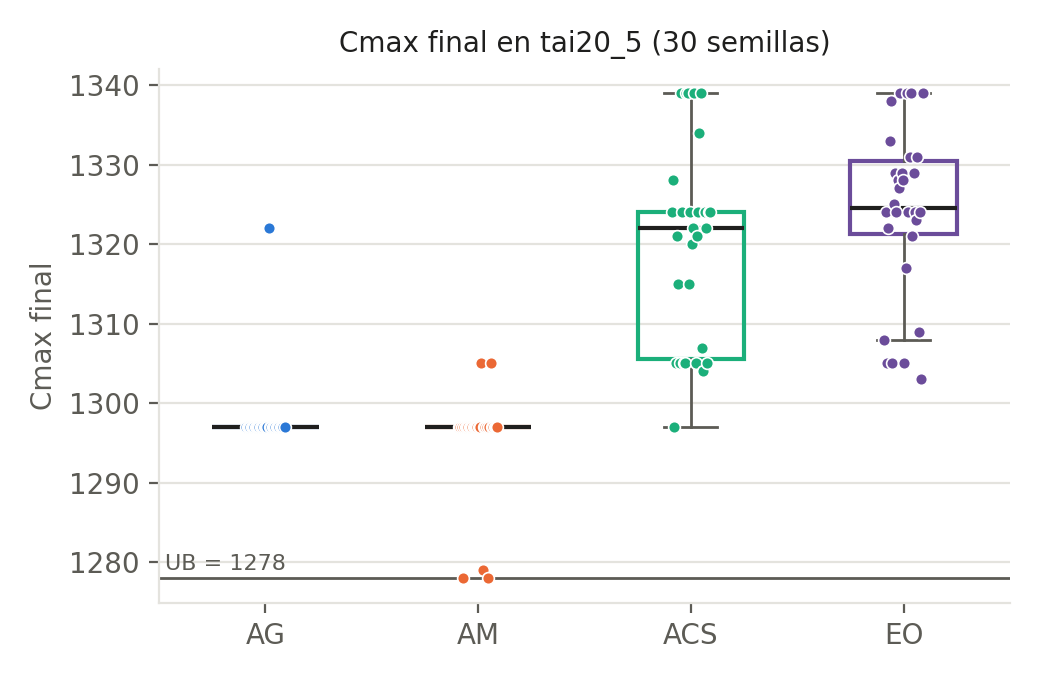
\includegraphics[width=\linewidth]{graficos/dispersion_tai20_5.png}
    \captionof{figure}{$C_{\max}$ final en ta001, 30 semillas.}\label{fig:disp20}
  \end{minipage}\hfill
  \begin{minipage}[t]{0.32\textwidth}\centering
    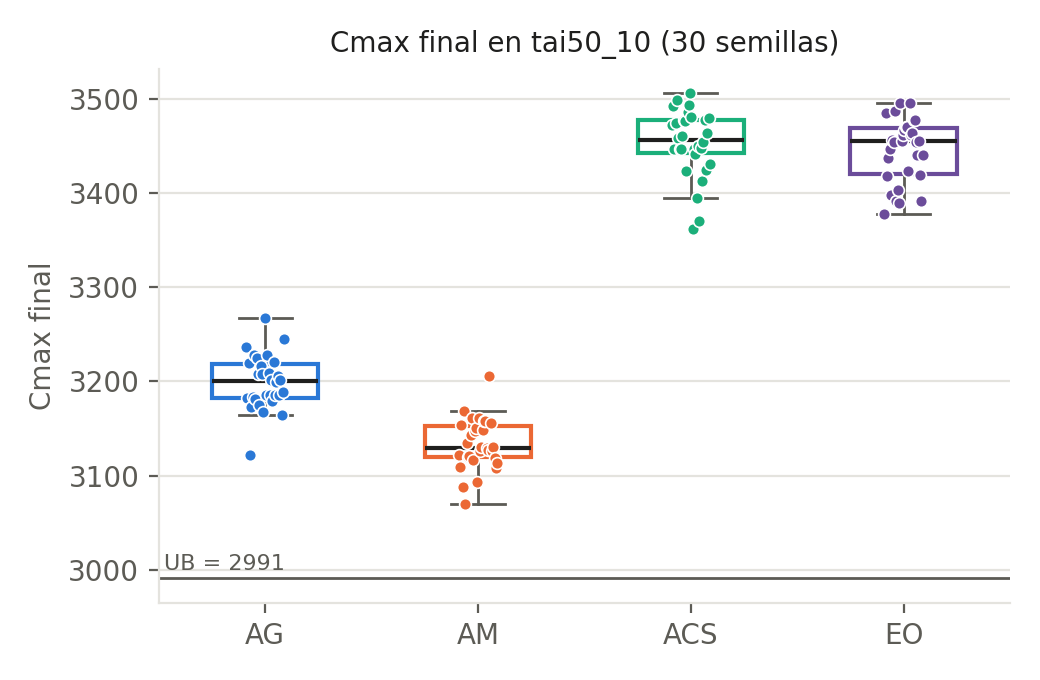
\includegraphics[width=\linewidth]{graficos/dispersion_tai50_10.png}
    \captionof{figure}{$C_{\max}$ final en ta041, 30 semillas.}\label{fig:disp50}
  \end{minipage}\hfill
  \begin{minipage}[t]{0.32\textwidth}\centering
    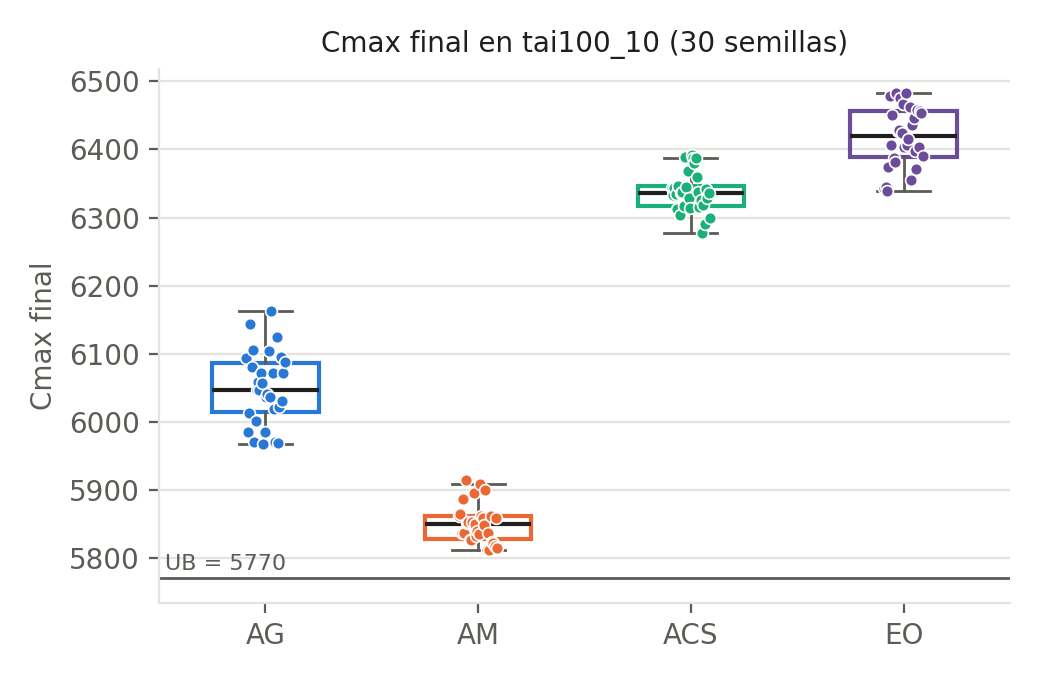
\includegraphics[width=\linewidth]{graficos/dispersion_tai100_10.png}
    \captionof{figure}{$C_{\max}$ final en ta071, 30 semillas.}\label{fig:disp100}
  \end{minipage}
\end{figure*}

\subsection{Líneas de base}
La Tabla~\ref{tab:base} responde de dónde salen las referencias. SPT es el \textit{makespan} de ordenar los trabajos por suma de tiempos, con argsort estable. La fila aleatoria es la media de 1\,000 permutaciones con el generador \texttt{Random(0)}, la misma muestra para cualquier semilla de los algoritmos. El RPD usa \eqref{eq:rpd} y la UB de la Tabla~\ref{tab:calidad}.

\begin{table}[!t]
  \caption{Líneas de base, una por instancia.}\label{tab:base}
  \centering\footnotesize
  \begin{tabular}{l l r r}\hline
    Instancia & Referencia & $C_{\max}$ & RPD (\%)\\ \hline
    ta001 & SPT & 1472 & 15.18\\
    & Aleatoria, media & 1516.2 & 18.64\\ \hline
    ta041 & SPT & 3781 & 24.99\\
    & Aleatoria, media & 3836.3 & 26.82\\ \hline
    ta071 & SPT & 6823 & 18.25\\
    & Aleatoria, media & 6923.8 & 20.00\\ \hline
  \end{tabular}
  \notatabla{SPT: un \textit{makespan}. Aleatoria: media de 1\,000 permutaciones, \texttt{Random(0)}. RPD respecto de la UB de la Tabla~\ref{tab:calidad}.}
\end{table}

Sobre esa media aleatoria, el ACS baja el RPD en 15.4, 12.7 y 10.2 puntos porcentuales (ta001, ta041 y ta071). EO baja 15.0, 12.9 y 8.8. SPT sola queda en 15.18\%, 24.99\% y 18.25\%, cerca del azar. Eso se observa. Una lectura posible, no demostrada aquí, es que el tiempo total de un trabajo dice poco sobre si conviene programarlo después de otro, porque el \textit{makespan} depende del acople entre máquinas.

\subsection{Convergencia y costo}
Las Figuras~\ref{fig:conv20}--\ref{fig:conv100} promedian, sobre 30 semillas, el mejor $C_{\max}$ contra las evaluaciones, en escala log. El eje común deja ver que el AM sigue después de $10^4$ evaluaciones.

\begin{figure}[!t]
  \centering
  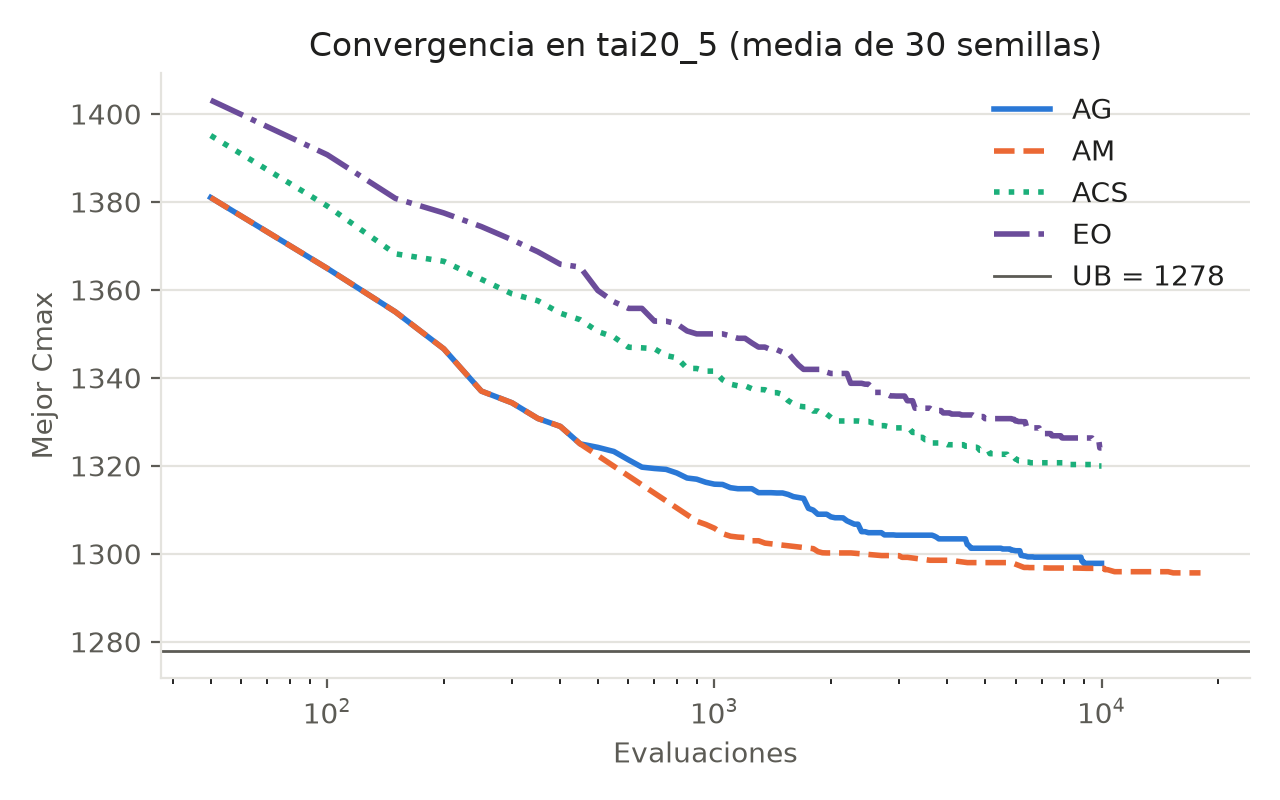
\includegraphics[width=\columnwidth]{graficos/convergencia_tai20_5.png}
  \caption{Convergencia media en ta001. La línea horizontal es la UB.}\label{fig:conv20}
\end{figure}
\begin{figure}[!t]
  \centering
  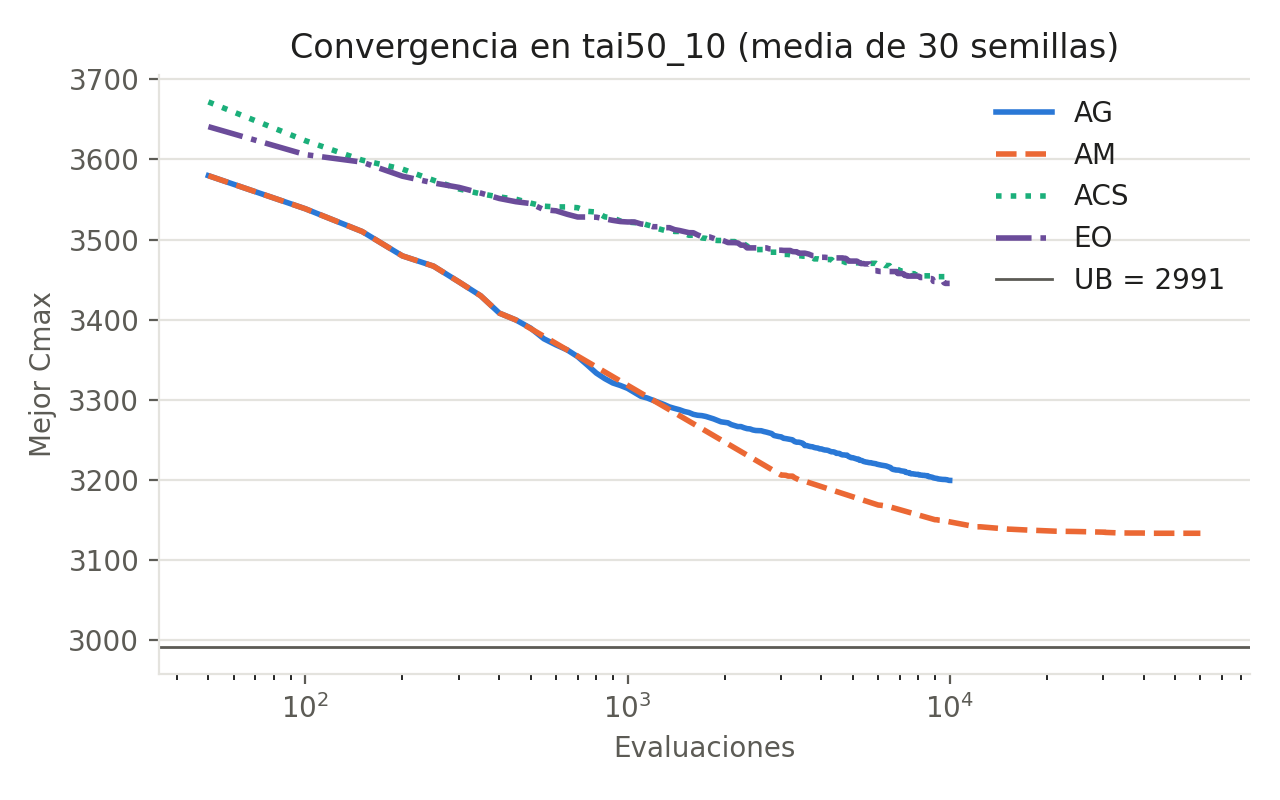
\includegraphics[width=\columnwidth]{graficos/convergencia_tai50_10.png}
  \caption{Convergencia media en ta041.}\label{fig:conv50}
\end{figure}
\begin{figure}[!t]
  \centering
  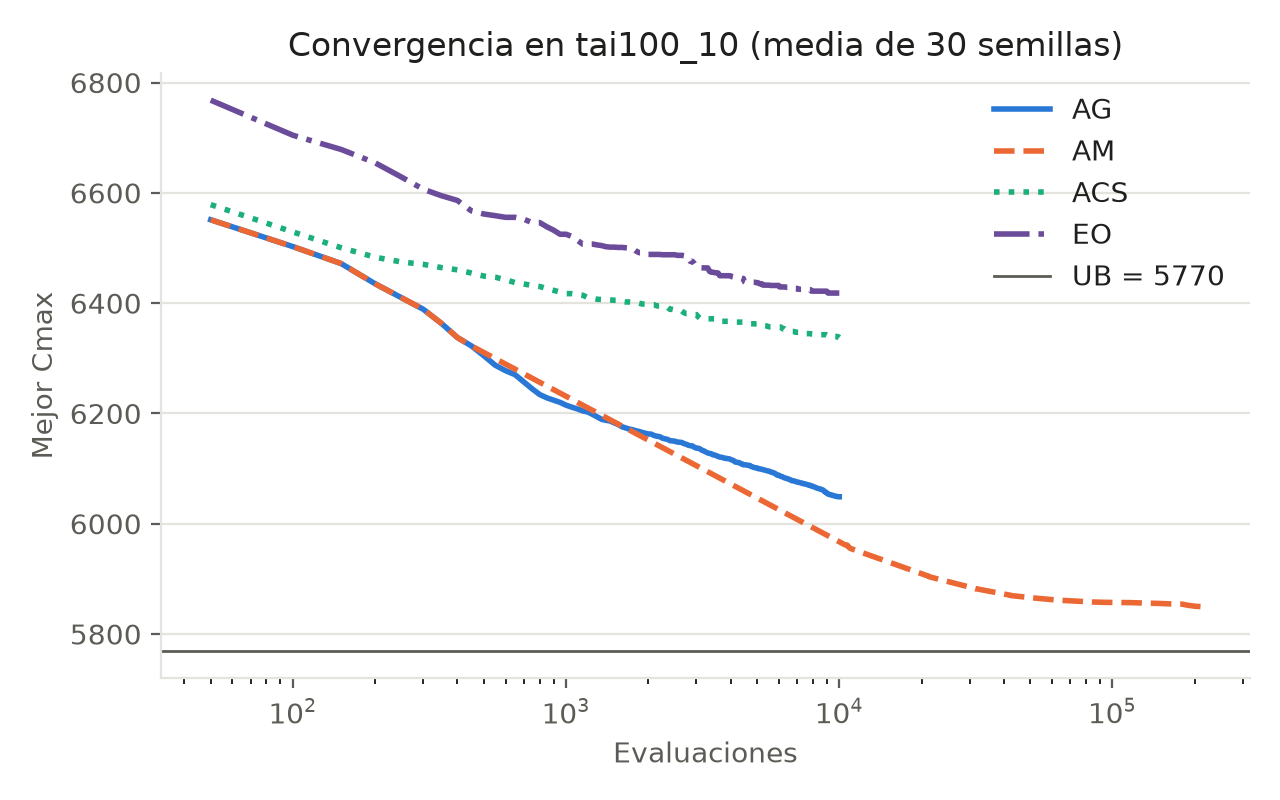
\includegraphics[width=\columnwidth]{graficos/convergencia_tai100_10.png}
  \caption{Convergencia media en ta071. El AM continúa tras $10^{4}$ evaluaciones.}\label{fig:conv100}
\end{figure}

AG y AM comparten semilla y ciclo hasta la primera búsqueda local, así que sus curvas coinciden al principio y se separan en la primera pasada. Después el AM baja en escalones. El AG sigue descendiendo cerca del final del presupuesto en ta041 y ta071. ACS y EO bajan más lento y se quedan por encima del AG. EO no tiene población ni feromona: solo reubica el trabajo ocioso elegido con la ley de potencia.

\begin{table}[!t]
  \caption{Costo por corrida, media de 30 semillas.}\label{tab:tiempo}
  \centering\footnotesize
  \begin{tabular}{l l r r r}\hline
    Instancia & Alg. & CPU (s) & Evaluaciones & Hallazgo\\ \hline
    $20\times5$ & AG & 1.16 & 10\,000 & 2\,280\\
    & AM & 1.82 & 18\,020 & 2\,685\\
    & ACS & 9.00 & 10\,000 & 3\,463\\
    & EO & 1.67 & 10\,000 & 5\,053\\ \hline
    $50\times10$ & AG & 3.92 & 10\,000 & 7\,515\\
    & AM & 21.18 & 60\,020 & 15\,517\\
    & ACS & 27.70 & 10\,000 & 5\,172\\
    & EO & 7.52 & 10\,000 & 5\,685\\ \hline
    $100\times10$ & AG & 8.01 & 10\,000 & 8\,707\\
    & AM & 147.58 & 210\,020 & 94\,186\\
    & ACS & 60.07 & 10\,000 & 6\,127\\
    & EO & 13.89 & 10\,000 & 4\,340\\ \hline
  \end{tabular}
  \notatabla{CPU: tiempo de procesador medio por corrida. Evaluaciones: columna homónima del resumen; en el AM incluye $20(n^2+1)$. Hallazgo: evaluación media en la que el registro alcanza el $C_{\max}$ final. La granularidad es una generación del AG o 50 iteraciones de EO.}
\end{table}

La Tabla~\ref{tab:tiempo} separa el costo del resultado. En ta071 el AM hace 210\,020 evaluaciones y tarda 147.58\,s; el AG hace 10\,000 y tarda 8.01\,s. Se observa que el AM tiene mejor RPD y más evaluaciones. No se separó cuánto de esa diferencia viene del presupuesto extra y cuánto del mecanismo de inserción: no hubo una corrida del AG con 210\,020 evaluaciones. El ACS gasta las mismas 10\,000 evaluaciones que el AG y tarda más (60.07\,s frente a 8.01\,s en ta071), porque cada hormiga recorre los trabajos pendientes. EO, con el mismo presupuesto base, tarda 13.89\,s en esa instancia y su hallazgo medio está en la evaluación 4\,340, antes que el del AG (8\,707), pero en un $C_{\max}$ peor (Tabla~\ref{tab:calidad}).

En el informe con siembra NEH y reemplazo $(\mu+\lambda)$ \cite{equipo_ag_neh_2026} el AG obtuvo RPD medios de 0.61\%, 3.24\% y 1.23\%, con otra población y otra cantidad de generaciones. La comparación es solo cualitativa. Es compatible con la idea de que parte de aquella calidad venía de la solución inicial, no solo del ciclo. No lo demuestra.

\section{Conclusiones}\label{sec:conclusiones}
En las tres instancias y con 30 semillas, el AM tiene el menor RPD medio. Es el único que iguala una UB, en 2 de 30 corridas de ta001. También es el que más evalúa: en $100\times10$, 21 veces las evaluaciones del AG. Esa ventaja de calidad y ese costo extra se observan juntos. Atribuir la calidad solo a la búsqueda local, o solo al presupuesto, exigiría igualar las evaluaciones.

ACS y EO, sin búsqueda local, quedan detrás del AG. Del ACS se conservó el ciclo de construcción y las dos actualizaciones; se adaptaron el grafo, la visibilidad SPT y el objetivo. La actualización local acerca $\tau$ a $\tau_0$ y no siempre la disminuye. EO acepta todo movimiento y solo archiva el mejor estado. Con $\tau=1.4$ no alcanza al AG.

Como trabajo futuro cabe dar a EO la misma pasada de inserción del AM, y combinar la colonia con esa búsqueda sobre la mejor hormiga. También cabe repetir el AG con el presupuesto de evaluaciones del AM, para separar costo y mecanismo.

\bibliographystyle{IEEEtran}
\bibliography{referencias}
\end{document}
